\documentclass[10pt]{article}

% Default 
\usepackage{graphicx}
\usepackage[backend=biber,
  style=numeric, 
  sorting=none]{biblatex}

% Additional
\usepackage{amsmath}
\usepackage{textcomp, gensymb}
\usepackage{placeins}
\usepackage{tabularray} 
\usepackage{xcolor}
\usepackage{placeins}
\usepackage{csquotes} 
\usepackage{todonotes} 

\newcommand{\td}[1]{\todo[linecolor=blue, backgroundcolor=blue!25,bordercolor=blue, size=\small, inline]{#1}}

\addbibresource{references.bib}

\title{Michelson Interferometer} 
\author{Rahmanyaz Annyyev, Hikmat Gulaliyev}
\date{28 April, 2024} 

\begin{document}

\maketitle

\begin{abstract}
  
\end{abstract}

\section{Introduction}

\subsection*{General}

A Michelson interferometer is an instrument used in optical interferometry to produce interference fringes. Minimally, it consists of two mirrors $M_1$ and $M_2$ and a beam splitter $M$ (although a diffraction grating can be used). The setup is shown in Figure \ref{fig:1}. The beam splitter, in our case, is a plate beamsplitter with a partially reflective coating. A source of light, $S$, a laser in our case, is directed at the beam splitter, and the light is split into two beams at point $C$. One beam is reflected toward mirror $M_1$, and the other one is transmitted toward mirror $M_2$. The beams are reflected by the mirrors and recombined at the beam splitter at point $C'$. The recombined beams are then directed to a screen, where they produce interference fringes.

\begin{figure}[hbt!]
  \centering
  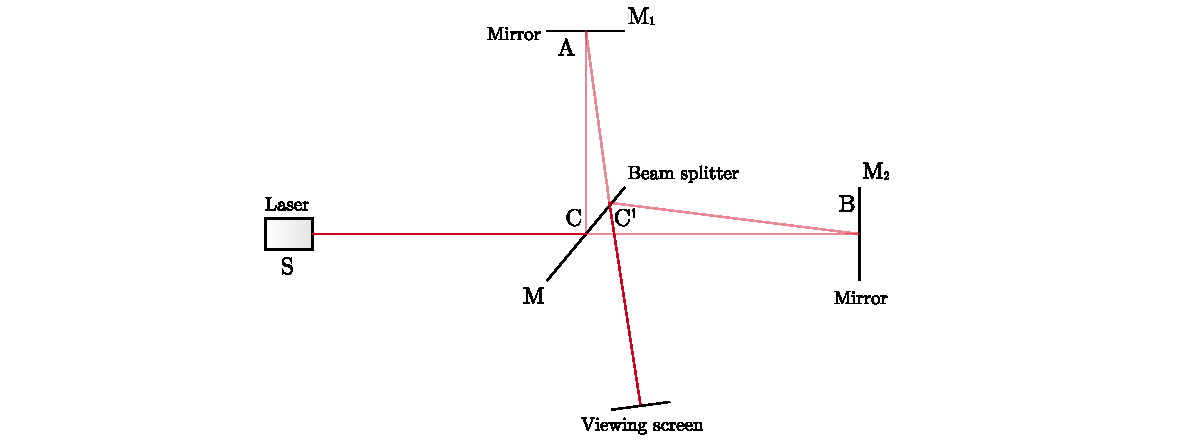
\includegraphics[scale=0.6]{figures/f1.pdf}
  \caption{The experimental setup of the experiment.}
  \label{fig:1}
\end{figure}





The Michelson interferometer is named after American physicist Albert Abraham Michelson, who built and used the device in the 1880s.

\subsection*{Procedure}

The experiment is comprised of two parts: A and B. The setup consists of ...

\subsubsection*{Part A}

\subsubsection*{Part B}

\section{Data \& Results}

\section{Discussion \& Conclusion}

\subsection*{Errors}

\subsection*{Approximations}

\subsection*{Discrepancies}

\subsection*{Conclusion}

\section{Extra credit}

% \printbibliography

\end{document}